\chapter{Numerical testing}\label{numtest}
\section{The Enzo code}
Enzo is a multiphysics, parallel AMR application for simulating the
cosmological evolution and star formation written in a mixture of C++ and
Fortran, making use of the message-passing interface (MPI) libaries and the 
HDF5 data format. \citet{Norman2007} describes the newest version of the code in
detail. In the following we summarize the most important features of the code.

Enzo simulates the evolution of dark and baryonic matter in a self-consistent
way on cosmological scales. Baryonic matter is evolved using a finite volume
discretization of the compressible fluid dynamic equations in comoving
coordinates\footnote{See appendix \ref{UEcomoving}.}. The Piecewise Parabolic
Method (PPM) in dual energy formalism for high Mach number flows is used to
integrate these equations \citep{Bryan1995}. Energy source and
sink terms due to
radiative heating and cooling processes are included, but not used in our work.
Also we do not use the multi-species (H, H+, He, He+, He++ and e-) capabilities
of Enzo; instead we always set the gas to be fully ionized with a mean
molecular
weight $m_{\mu}= \unit[0.6]{u}$. Dark matter is assumed to behave as
collisionless fluid, obeying the Vlasov-Poisson system of
equations\footnote{See appendix \ref{vlaspois}.}. Its evolution is
solved using particle-mesh algorithms for collisionless N-body dynamics;
specifically a second order accurate Cloud-in-Cell (CIC) formulation with
leapfrog time integration is used. Dark matter and baryonic matter interact
through their
gravitational potential. The gravitational potential is computed by solving the
Poisson equation on the adaptive grid hierarchy using Fast Fourier Transform and
multigrid techniques. In generic terms, Enzo is a fluid solver for the baryonic
matter coupled to a particle-mesh solver for the dark matter via a Poisson
solver. The coordinates of the simulation domain are given as comoving
coordinates in an expanding universe with a scale factor $a(t)$, which is
computed as a solution of the Friedman equation.

The code uses blockstructured adaptive mesh refinement (as described in 
section \ref{amr}) to achieve high resolution. To parallelize the computation,
a concept of ghost grids is used. The root grid is split into a number of grid
patches, at least as many as the number of processors. Then, as grids
are added, each grid is placed by default on the same processor as its parent.
Once the rebuild of the hierarchy has been completed on a given level, the load
balancing ratio between processors is computed and grids are transfered between
processors in an attempt to even the load. However, the structure of the
grid patch hierarchy is stored redundantly on every processor to ease
communication. To allow for this, each real grid, which resides on only one
processor, is represented by a ghost grid (which is a grid patch without data)
on every other processor. This structure is shown graphically in figure
\ref{fig:ghost}. 

\begin{figure}[tp]
\centering
\includegraphics[width=0.7\linewidth]{chapter7/norman-f2.eps}
\caption{Real and ghost grids in a hierarchy; real and ghost zones in a grid 
\citep{Norman2007}.}
\label{fig:ghost}
\end{figure}

Enzo is publicly available from \url{http://lca.ucsd.edu/software/enzo/}.
However to integrate and test our SGS model several modifications to the public
version were necessary.

\section{Modifications to Enzo}
\subsection{Turbulent energy as a color field}
To implement the Schmidt model into Enzo, it was necessary to introduce a new
field for the turbulent energy, which is advected by the PPM solver. To achieve
this, we used the capability of Enzo to incorporate an arbitrary number of
color fields\footnote{See appendix \ref{color}.} into the simulation. Thus the
turbulent energy field is implemented as another color field. Nevertheless it
was necessary to change the default behavior of color fields in Enzo. By
default, Enzo treats a color like a density. But since we want turbulent energy
to be treated in analogy to the internal energy, which is implemented as
specific quantity, we changed the treatment of color fields in our version of
Enzo as to behave like a specific quantity.

\subsection{Coupling of turbulent energy and time step restriction}
The source/sink terms in the turbulent energy equation and the terms arising in
the internal energy equation and the momentum equation due to our subgrid model
are coupled to the fields in first order, which means for some arbitrary field
$f$ at timestep $t_n$, the source terms $s_1,s_2, \ldots$ are added in the
following way 
\begin{align}
f_{n+1} = f_n + s_{1,n} \Delta t + s_{2,n} \Delta t + \ldots
\end{align}
where $\Delta t = t_{n+1}-t_n $ is the chosen timestep. But due to the low
accuracy of the scheme, it might happen, that for a big timestep the value of
one of the energy fields in a cell drops below zero, which is unphysical and
numerically unstable. To account for that, we had to restrict the timestep in
the code. We do this by applying the following estimator
\begin{align}
\Delta t_{turb} = C_{turb} 
\min \lra{\sqrt{\frac{l_{\Delta}}{\abs{\vec{a}_{turb}}}}},
\end{align}
where the minimum is taken over all cells of all grids on one
level of refinement, the turbulent acceleration is $\vec{a}_{turb}=
\frac{1}{\fil{\rho}}{\pd{r_j}\hat{\tau}(v_i,v_j)}$ and $C_{turb} = 0.05$. If
the so-estimated minimal allowed timestep due to our turbulent model $
\Delta t_{turb}$ is smaller than the timestep computed by the other estimators
in the code (e.g. estimator based on the CFL-criterion, for gravity and so on) 
it will be chosen as the timestep for the next iteration. This procedure
ensures that even for big turbulent acceleration (which also means
big source/sink terms) due to our turbulent model, our computation is
numerically stable. Of course, there is one drawback to this procedure: if the
turbulent acceleration becomes really huge, the timestep of the simulation will
be extremely small, effectively stopping the simulation. This can only be
circumvented by either using a higher accuracy scheme for coupling the 
sink/source terms to the equations or by using a different subgrid model, which
does not produce numerically instable huge values of $\abs{\vec{a}_{turb}}$.
The Sarkar corrections are a step in this direction, but further steps may be
necessary in the future. 

\subsection{Transfer of turbulent energy at grid refinement/derefinement}
By default, when a new finer grid gets created in Enzo, the values on the finer
grid are generated by interpolating them from the coarser grid using a
conservative interpolation scheme. At each timestep of the coarse grid, the
values from the fine grid are averaged and replace the values computed on the 
coarse grid in the region where fine and coarse grid overlap. As already
mentioned in section \ref{epsilon} these procedures must be modified in our
approach to combine LES and AMR.

So at refinement we do the following:
\begin{enumerate}
\item Interpolate the values from the coarse to the fine grid using standard
interpolation scheme from Enzo.
\item On the finer grid, correct the values of specific kinetic energy 
$e_k= \frac{1}{2}v^2$, velocity components $v_i$ and specific turbulent energy
$e_t=\frac{1}{2}q^2$ as follows
\begin{align}
e'_k&=e_k+e_t \lra{1-r^{-2/3}},\\
v'_i&=v_i \sqrt{1+\frac{e_t}{e_k}\lra{1-r^{-2/3}}},\\
e'_t&=e_t-e_t\lra{1-r^{-2/3}},
\end{align}
where primed quantities are the final values on the fine grid.
\end{enumerate}

At derefinement we reverse this procedure:
\begin{enumerate}
\item Average the values from the fine grid and replace the corresponding values
on the coarse grid
\item On the coarse grid, correct the averaged values of kinetic energy, 
velocity components and turbulent energy
\begin{align}
e'_t&=e_t+e_t\lra{r^{2/3}-1},\\
v'_i&=v_i \sqrt{1-\frac{e_t}{e_k}\lra{r^{2/3}-1}},\\
e'_k&=e_k-e_t \lra{r^{2/3}-1}.
\end{align}
Here primed quantities denote the final values on the coarse grid. 
\end{enumerate}
It should be noted that derefinement with this procedure is only possible if
there is enough kinetic energy on the fine grid, because on the coarse grid, we
must have $e'_k \geq 0$. This is only the case for
\begin{align}
\frac{e_t}{e_k} \leq \lra{r^{2/3}-1}.
\end{align}
For example for a refinement ratio $r=2$ this yields $e_k \geq 0.58 e_t$.
So if this criterion is not satisfied, we do not correct the values of the
energies and velocities at derefinement.\footnote{One might ask, why not do
the correction step before the interpolation/averaging step, since that might
produce less noise. The reason for our choice was, that otherwise we would had
to introduce an additional temporary field into the code, which would lower
the performance.}

\subsection{Random forcing}\label{randforce}
To simulate driven turbulent flow, a random forcing mechanism was implemented
into our version of Enzo. The forcing field is generated by a stochastic
differential equation called Ornstein-Uhlenbeck process
\citep{Schmidt2004}. This 
process generates a temporally and spatially varying force field which acts on
the fluid. The components of the force are generated in Fourier space, because
there it is easier to split the force field into a solenoidal and a 
dilatational (compressive) part.\footnote{Also called Helmholtz decomposition,
see \citet{Schmidt2004}.} Hence the force field is characterized by a weight
$\zeta$, which is zero, if the force field is purely compressive (which means it
will not directly generate any vorticity), and one, if the force field
is purely solenoidal (which means it will not directly generate any
divergence in the velocity field). The strength of the force field is
characterized by a forcing 
Mach number $M_f$, which is loosely connected to the mean Mach number reached 
in the simulation after one integral time
\begin{align}
t_{int}=\frac{l_0}{M_f \fil{c_s}},
\end{align}
where $l_0$ is the mean driving length scale size and
$\fil{c_s}$ is the mean sound speed. The force field is adjusted to drive
the fluid only on length scales around the characteristic forcing length $l_0 =
\frac{l_{box}}{\alpha_f}$ with $\alpha_f =2 $ to allow for an
undisturbed generation of the energy dissipation cascade down to smaller
scales. 

\subsection{Statistics tool}
To be able to extract and analyze statistical quantities from the simulation,
sophisticated routines have been implemented, which allow us to compute 
mass weighted and normal mean values, standard deviations and root mean square
values at every cycle for each quantity and for each level of an AMR simulation.
We make heavy use of these routines in the following sections. 

\section{Energy conservation}\label{numenergy}
Global conservation of energy in a fluid code with a SGS model like the
Schmidt model is not achieved easily. This is because of the nonlocal features
of this model. As shown in chapter \ref{FE}, the equation of turbulent energy
\eqref{eq:etsum} is generated by subtracting the equation of resolved kinetic
energy \eqref{eq:filkinsum} from the filtered equation of turbulent energy
\ref{eq:filkin}. In other words, the sum of turbulent energy equation and
resolved energy equation must yield the filtered kinetic energy equation.
In particular, the sum of turbulent production term
$\hat{\tau}(v_j,v_i)\pd{r_j}\hat{v_i}$ and resolved kinetic energy reduction
term $\hat{v}_i\pd{r_j}\hat{\tau}(v_i,v_j)$ must add
up to the corresponding flux term in the filtered equation of kinetic energy
\begin{align}
\pd{r_j}\hat{v}_i\hat{\tau}(v_i,v_j) =
\hat{v}_i\pd{r_j}\hat{\tau}(v_i,v_j)+\hat{\tau}(v_j,v_i)\pd{r_j}\hat{v_i}.
\label{eq:fluxsum}
\end{align}
This is important, since we know that the integral of the flux term over the
whole volume must be zero
\begin{align}
\int \pd{r_j}\hat{v}_i\hat{\tau}(v_i,v_j) dV = 
\oint\hat{v}_i\hat{\tau}(v_i,v_j) dA = 0. \label{eq:globalflux}
\end{align}
But this is not guaranteed numerically, if we compute the turbulent production
term and the kinetic energy reduction term independent of each other, since
small numerical errors might lead to a violation of equation \eqref{eq:fluxsum}
locally, which leads to a big violation of equation \eqref{eq:globalflux}
globally.

We therefore compute the resolved kinetic energy reduction term indirectly as
\begin{align}
\hat{v}_i\pd{r_j}\hat{\tau}(v_i,v_j) = 
\pd{r_j}\hat{v}_i\hat{\tau}(v_i,v_j) - 
\hat{\tau}(v_j,v_i)\pd{r_j}\hat{v_i},
\end{align}
since this will guarantee, that equation \eqref{eq:globalflux} is fullfilled
globally. We found that the global energy is thus much better conserved. 

In the following we present our results on energy conservation. The analyzed
simulation of driven turbulence has a static grid of size 1.0 (in code units)
with a resolution of $256^3$ grid points and periodic boundary conditions. At
time $t=0$ the baryonic fluid is at rest. The fluid is driven by random forcing
as described in section \ref{randforce} with $\zeta = 1.0$ and $M_f = 0.68$. The
simulation is adiabatic (the adiabatic index $\gamma=\frac{5}{3}$) and uses none
of the features
necessary for a cosmological simulation (comoving coordinates, selfgravity, dark
matter \ldots) except dual energy formalism. The mean sound speed of the
simulation is $c_s=\sqrt{\gamma}$, since the mean pressure and density are set
to one in code units. 

\begin{figure}[tp]
\centering
\subfigure[No SGS model.]{
\includegraphics[width=0.45\linewidth]{chapter7/energynosgs2.eps}
\label{fig:nosgs}}
\subfigure[Schmidt model.]{
\includegraphics[width=0.45\linewidth]{chapter7/energysgs2.eps}
\label{fig:sgs}}
\caption{Mass weighted mean energies over time in driven turbulence simulation.}
\end{figure}

The plots \ref{fig:nosgs} and \ref{fig:sgs} show the typical time development of
the mass weighted mean energies in our simulation including the energy injected
into the system by random forcing. It is evident from the curve of the turbulent
energy, that after one integral time scale, our simulation reaches a equilibrium
between production and dissipation of turbulent energy.

\begin{figure}[tp]
\centering
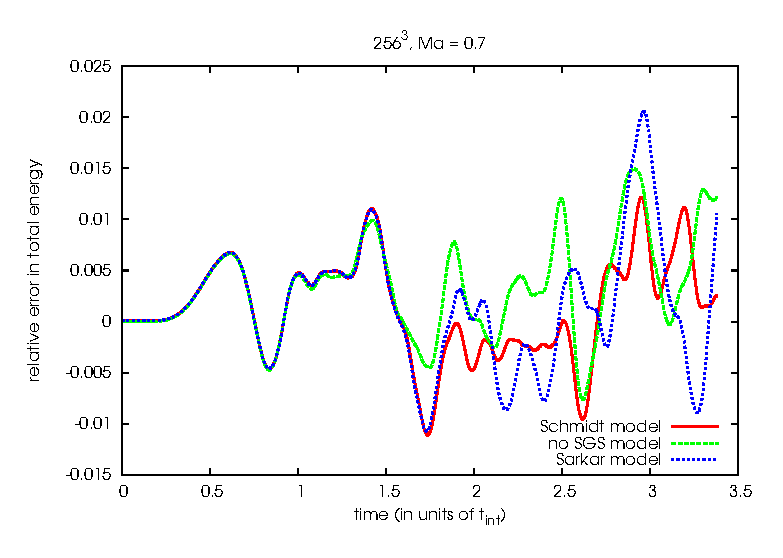
\includegraphics[width=0.7\linewidth]{chapter7/relerror2.eps}
\caption{Relative error of total energy in the simulation.}
\label{fig:relerror}
\end{figure}

In figure \ref{fig:relerror} we plotted the time development of the relative
error $\frac{\Delta e(t)}{e(0)}$ of the mean total energy,
which is the sum of the mass weighted means of internal energy, kinetic energy,
turbulent energy minus the injected energy due to the forcing
\begin{align}
\hat{e}_{tot}= \hat{e}_{int}+\hat{e}_{kin}+\hat{e}_t-\hat{e}_f, 
\end{align}
where $\hat{e} = \frac{\fil{\rho e}}{\fil{\rho}}$. It demonstrates, that with
our Schmidt model, the relative error in energy is comparable to the error
without SGS model and is around 1\%. Also the energy conserving properties of
the Sarkar model are equally good. 

\begin{figure}[tp]
\centering
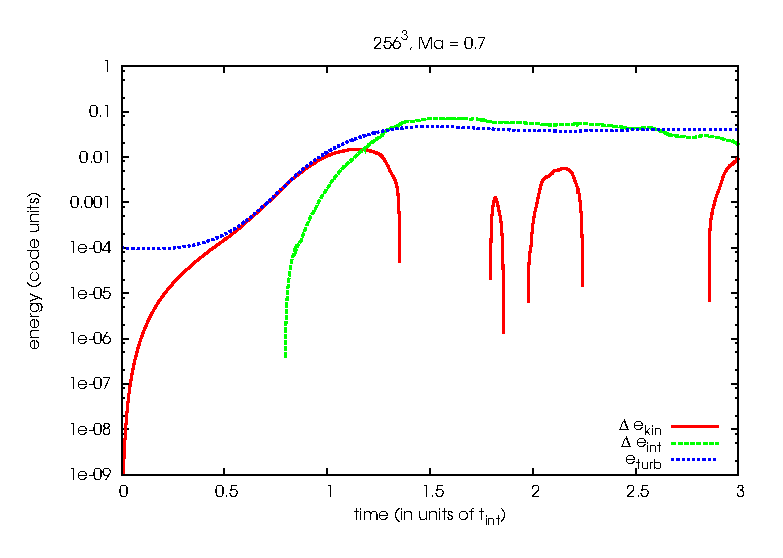
\includegraphics[width=0.7\linewidth]{chapter7/diffenergy2.eps}
\caption{Differences in energies between simulation with and without SGS model,
compared to the time development of the turbulent energy.}
\label{fig:diffenergy}
\end{figure}

It is also instructive to plot the difference between internal energy of the
simulation without the SGS model and the internal energy with the Schmidt model
and the
difference between the kinetic energies of both simulations. These differences
are shown in figure \ref{fig:diffenergy}. One can conclude from this figure,
that, at the beginning of the turbulent driving, the turbulent energy produced
in our simulation with SGS is found in the kinetic energy of the
simulation without SGS. From $t=1.2\ t_{int}$ on most of the turbulent energy
can be found in the internal energy of the simulation without SGS.
Turbulent energy can therefore be interpreted as a kind of buffer, which
prevents the kinetic energy in our simulation to be converted instantly into
thermal energy.  

\section{Scaling of turbulent energy}\label{eturbscale}
In our $\epsilon$-based approach to combine AMR and LES we assumed that the
turbulent energy scales according to equation $\eqref{eq:qscale}$ like
$q^2 \sim l^{2/3}$. We conducted several simulations of driven turbulence to
check the validity of this assumption.

The simulations were done on a static grid in a computational domain of size
1.0 with periodic boundary conditions. At
time $t=0$ the baryonic fluid is at rest. The fluid is driven by random forcing
as described in section \ref{randforce} with $\zeta = 0$ (purely solenoidal
forcing). The simulations were done for nearly isothermal gas
($\gamma=1.01$) with mean pressure and density set to $1.0$ in code units.
We used forcing Mach numbers of $M_f=0.2$ and $M_f=0.68$ and varied the
resolution from $32^3$ to $256^3$ grid points. For $M_f=0.68$ the simulations
were transonic reaching reaching a Mach number around one (see figure
\ref{fig:mach}).

\begin{figure}[tp]
\centering
\includegraphics[width=0.7\linewidth]{chapter7/mach2.eps}
\caption{Mean Mach number for adiabatic and isothermal simulation using an
equal
forcing Mach number $M_f=0.68$.}
\label{fig:mach}
\end{figure}

The characteristic time development of the turbulent energy dependent on the
resolution of the simulation can be seen in figures \ref{fig:mf2schmidt} -
\ref{fig:mf7sar}. 

\begin{figure}[tp]
\centering
\subfigure[Schmidt model, $M_f=0.2$.]{
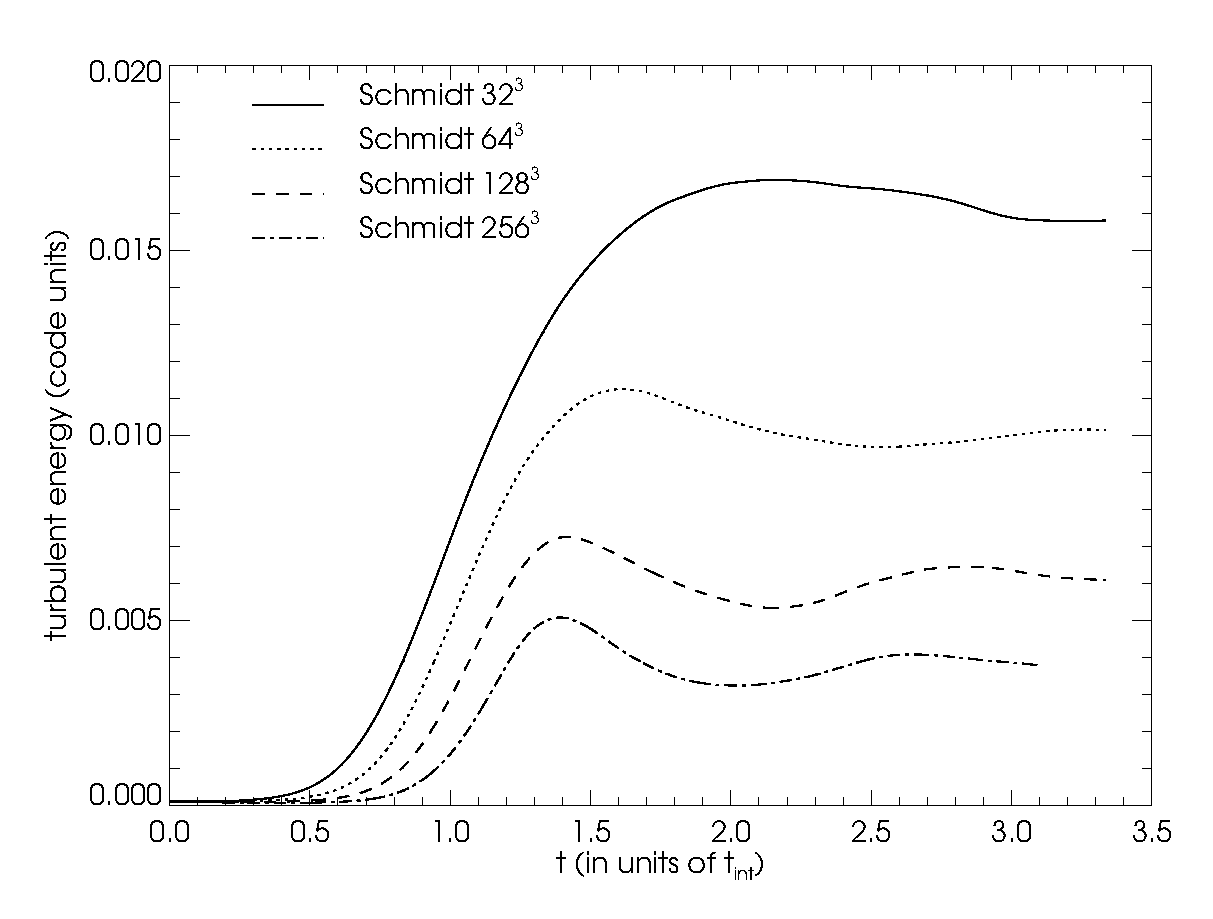
\includegraphics[width=0.45\linewidth]{chapter7/tueres2schmidt.eps}
\label{fig:mf2schmidt}}
\subfigure[Sarkar model, $M_f=0.2$.]{
\includegraphics[width=0.45\linewidth]{chapter7/tueres2sar.eps}
\label{fig:mf2sar}}
\subfigure[Schmidt model., $M_f=0.7$]{
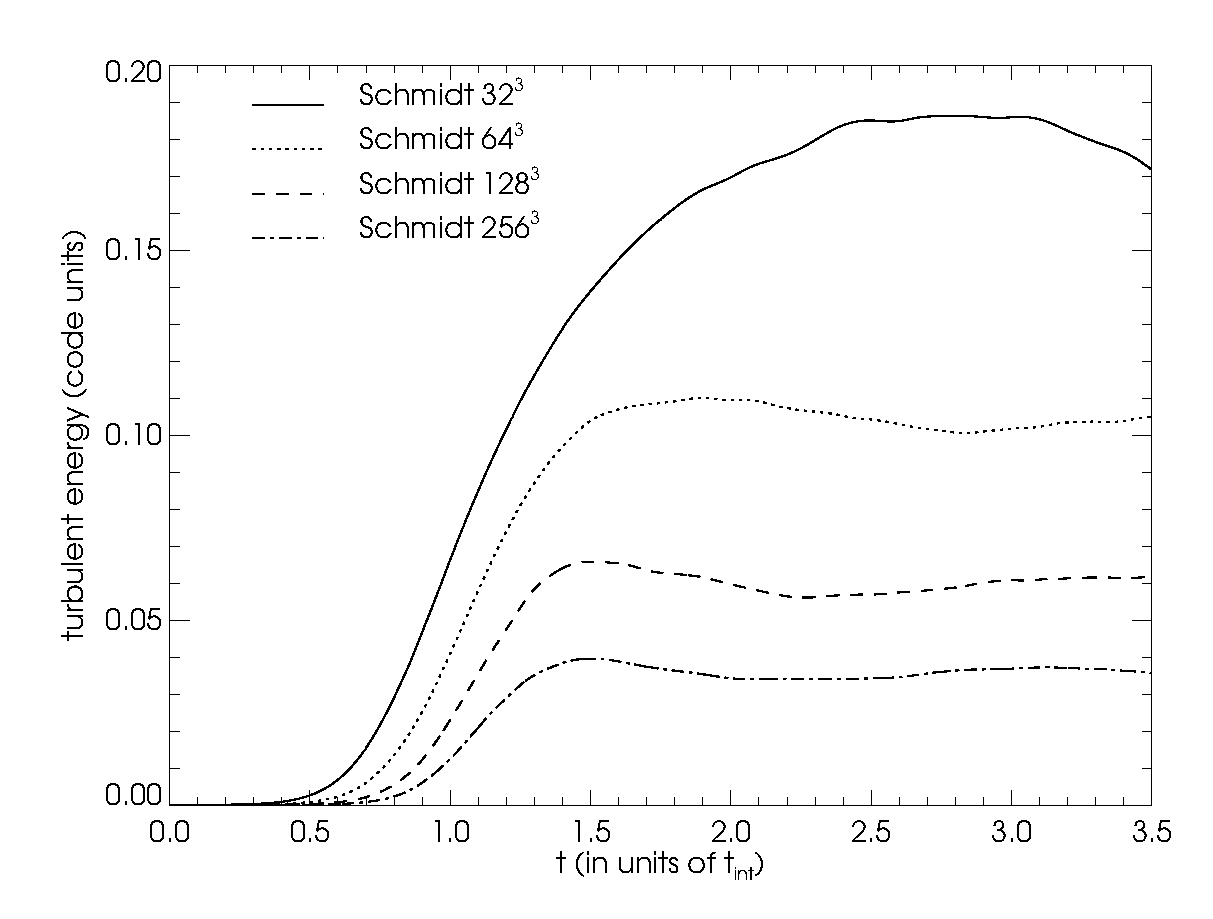
\includegraphics[width=0.45\linewidth]{chapter7/tueres7schmidt.eps}
\label{fig:mf7schmidt}}
\subfigure[Sarkar model, $M_f=0.7$.]{
\includegraphics[width=0.45\linewidth]{chapter7/tueres7sar.eps}
\label{fig:mf7sar}}
\caption{Mass weighted mean turbulent energies over time in driven turbulence
simulation, for resolutions $32^3$ to $256^3$ with forcing Mach number $M_f=0.2$
and $M_f=0.68$.}
\end{figure}

We compute mean turbulent energies by
averaging the turbulent energy from $t=3.0\ t_{int}$ to the end of the
simulation
and plot them against the resolution of the simulation. The results together
with a power-law fit are shown in figures \ref{fig:tuefit2} and
\ref{fig:tuefit7}. 
From this we see that for a low Mach number forcing our assumption  
$q^2 \sim l^{2/3}$ ($l$ is indirect proportional to the resolution) is fulfilled
indeed. Nevertheless for high Mach number flows the scaling of turbulent energy
becomes steeper and is $q^2 \sim l^{0.77}$ for the Schmidt model and 
$q^2 \sim l^{0.71}$ for the Sarkar model. In other words for
higher Mach number flows, our correction of turbulent energy at grid 
refinement/derefinement based on relation $\eqref{eq:qscale}$ should probably
be seen only as a good guess of the initial values of turbulent energy on
the finer/coarser grid. Also we conclude that for higher Mach number flows one
should use the Sarkar corrections to the Schmidt model, since this leads
to a scaling of turbulent energy more similar to the incompressible low Mach
number case. 

\begin{figure}[tp]
\centering
\subfigure[$M_f=0.2$.]{
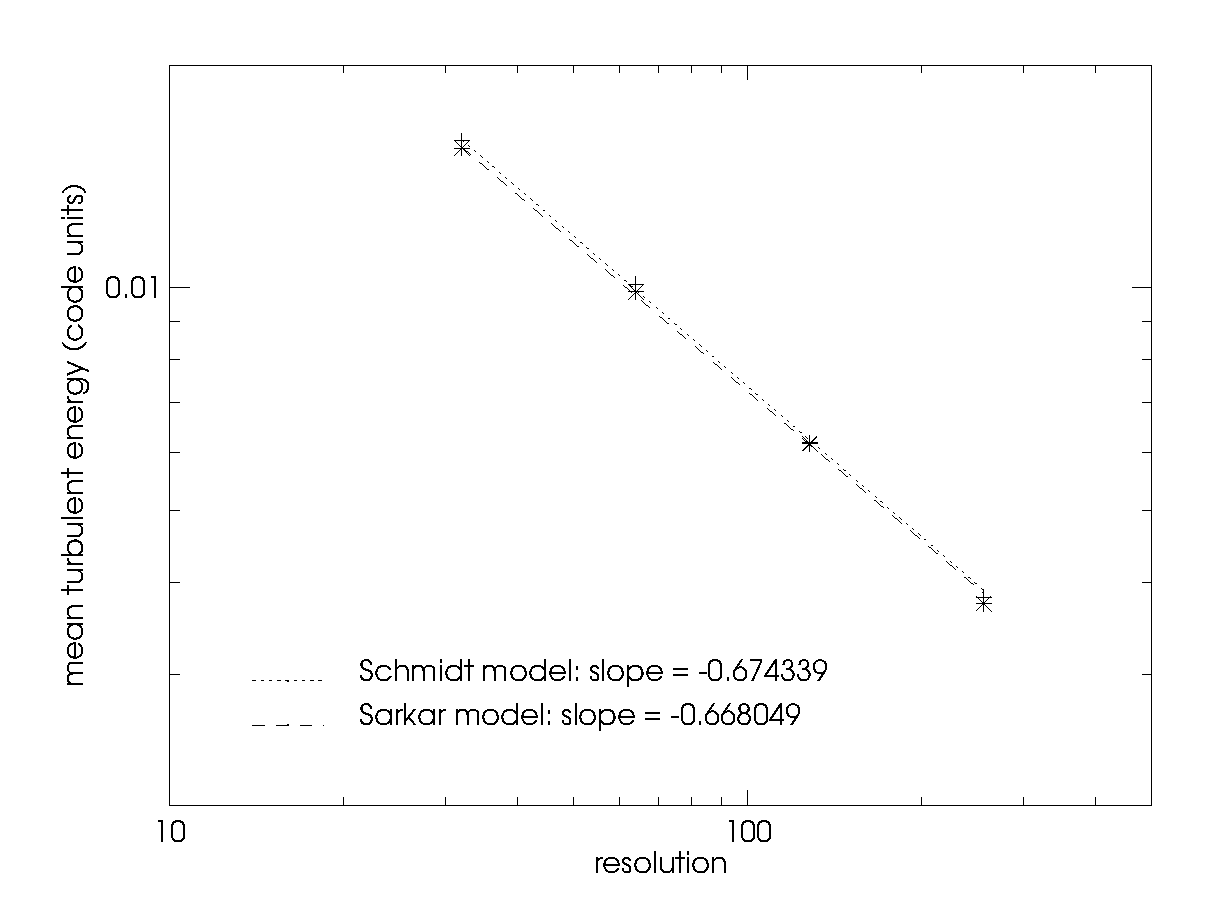
\includegraphics[width=0.45\linewidth]{chapter7/tuefit2.eps}
\label{fig:tuefit2}}
\subfigure[$M_f=0.68$.]{
\includegraphics[width=0.45\linewidth]{chapter7/tuefit7.eps}
\label{fig:tuefit7}}
\caption{Scaling of turbulent energy dependent on resolution for different
strength of the forcing.}
\end{figure}

\section{Comparison of static grid to AMR turbulence simulations}

\begin{figure}[p]
\centering
\includegraphics[width=0.7\linewidth]{chapter7/eturbamr27trs2sar.eps}
\caption{Thick lines: mean mass weighted turbulent energy for each level of the
 AMR simulation using our procedure of transferring turbulent energy at grid
refinement/derefinement. Thin lines: the corresponding development of turbulent
energy of the static grid simulations.}
\label{fig:amrtrs2}
\end{figure}

\begin{figure}[p]
\centering
\includegraphics[width=0.7\linewidth]{chapter7/eturbamr27trs0sar.eps}
\caption{Thick lines: mean mass weighted turbulent energy for each level of the
 AMR simulation without transferring turbulent energy at grid 
refinement/derefinement. Thin lines: the corresponding development of turbulent
energy of the static grid simulations.}
\label{fig:amrtrs0}
\end{figure}

To be consistent the results of an AMR simulation in the limit of
complete refinement of the whole computational domain should resemble the
results of a corresponding static grid simulation. To test this, we compared
an AMR simulation with a $32^3$ root grid resolution and three additional
levels with a refinement factor of 2 between each level, covering the whole
domain, with the corresponding static grid simulations of driven turbulence with
resolutions of $32^3,64^3,128^3$ and $256^3$. 

Again the simulations were done in a computational domain of size 1.0 with
periodic boundary conditions. At time $t=0$ the baryonic fluid is at rest. The
fluid is driven by random forcing as described in section \ref{randforce} with
$\zeta = 0$ (purely solenoidal
forcing). The simulations were done for nearly isothermal gas
($\gamma=1.01$) with mean pressure and density set to $1.0$ in code units.
We used a forcing Mach number of $M_f=2.7$ and therefore used the SGS model
with Sarkar corrections. 


The results of this consistency check can be seen in figure \ref{fig:amrtrs2}.
We observe that the time development of the mean turbulent energy in this
simulation of supersonic driven turbulence simulation is very similar on the
different levels of the AMR simulation compared with the static grid
simulations, except for some deviations at the root level. But comparing these 
results to a simulation without correcting turbulent energy at grid
refinement/derefinement (figure \ref{fig:amrtrs0}), it is evident that our
$\epsilon$-based approach of turbulent energy transfer is much more consistent
with the static simulations of driven turbulence. 
